%!TEX root = ../ausarbeitung.tex
\newpage
\section{Klassifizierung mit Histograms of Gradients und Support Vector Machines} \label{sec:HOG}


\subsection{Einführung zu Histograms of Oriented Gradients} \label{ssec:intro_HOG}

Die Bezeichnung \textit{Histograms of Oriented Gradients} (HOG) bezeichnet einen \textit{Feature Descriptor} und wurde bekannt durch die Arbeit von Navneet Dalal and Bill Triggs \cite{dalal05}. Initial wurde der Deskriptor verwendet um Fußgänger zu detektieren. Später wurde er auch für andere Objekte wie Autos, Busse und Tiere eingesetzt. Wie der Name bereits andeutet handelt es sich bei HOG um ein Histogramm basierten \textit{Feature Descriptor}. Die Berechnung des HOG-Descriptors lässt sich in drei Schritte unterteilen: Gradientenberechnung, Gruppierung der Orientierungen und Histogrammerzeugung. Häufig werden  auch Vorverarbeitungsschritte, wie zum Beispiel ein Histogrammausgleich durchgeführt.

Zur Gradientenberechnung wird der Sobel-Operator verwendet. Eine visuelle Darstellung des Ergebnisses ist in Abbildung~\ref{fig:sobel} gezeigt. Zu sehen ist die Magnitude der Ableitung über die vertikale (links) und horizontale (rechts) Bildachse. Dabei entspricht in dieser Darstellung der Grauwert der positiv definierten Magnitude des Gradienten. Mit den folgenden Formeln lassen sich aus den Beiden Gradienten die positiv definierte gesamt Magnitude $|G|$ und die Orientierung $\Theta$ berechnen:  

\begin{equation}
|G| = \sqrt{G_x^2 + G_y^2}
\end{equation}
\begin{equation}
\Theta = \arctan({G_x, G_y})
\end{equation}

\begin{center}
\begin{tabular}{c}
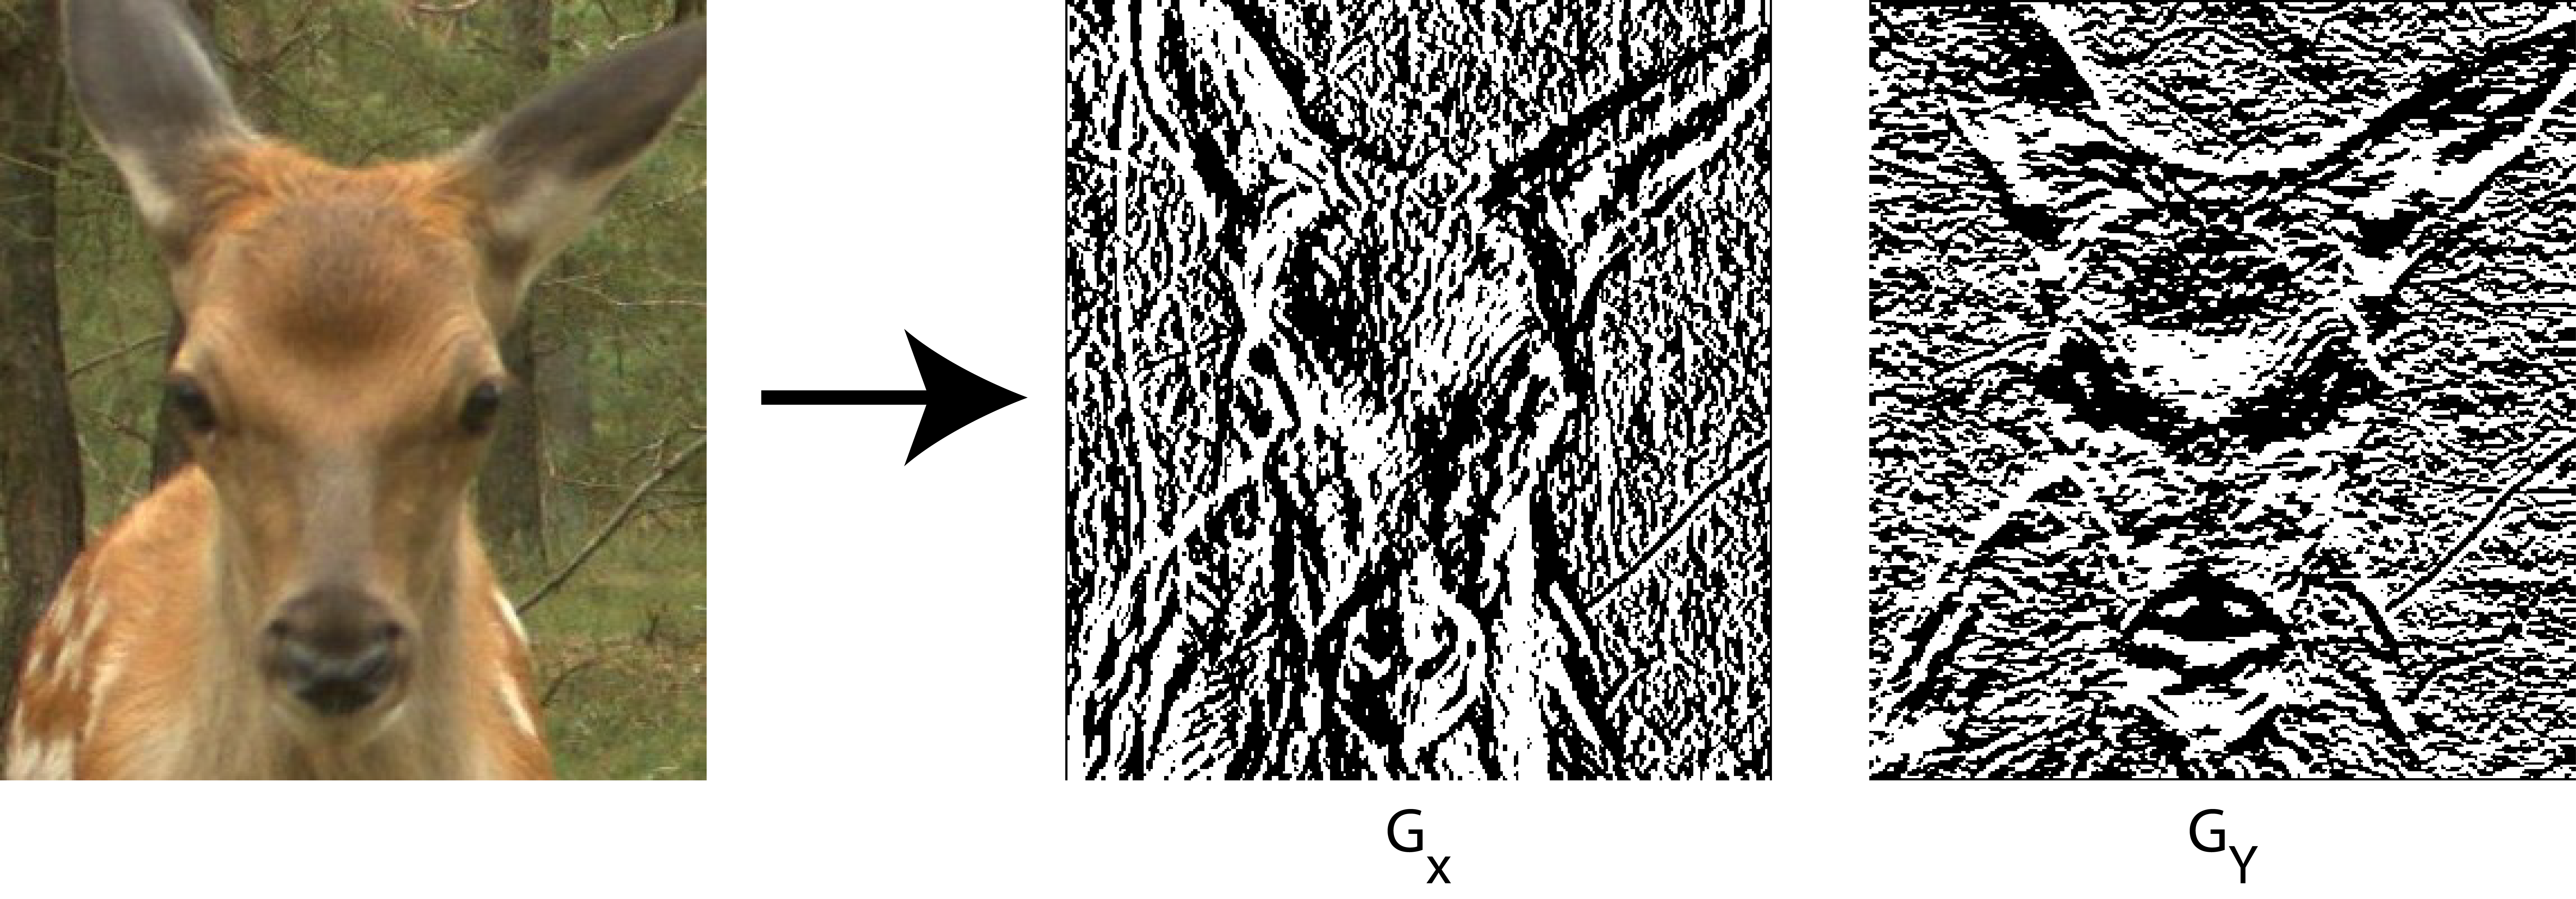
\includegraphics[trim={0 0cm 0cm 0cm},clip=true,width=13cm]{img/sobel.png}
\end{tabular}
\captionof{figure}{Exemplarische Ergebnisbilder des Sobel-Operators für die vertikale und horizontale Bild Achse. Die Grauwerte entsprechen der Magnitude des Gradienten.}
\label{fig:sobel}
\end{center}

Für jeden Pixel eines Bildes wird die Magnituden und Orientierung berechnet. Anschließend werden sie entsprechend ihrer Orientierung in gleich Gruppen sortiert. Häufig wird die Richtung der Orientierung ignoriert und 9 Gruppen verwendet. Durch das Ignorieren der Richtung wird also nur ein halber Kreis betrachtet (0 - 180°). Bei 9 Gruppen bedeutet dies, dass jede Gruppe 20° abdeckt. Der Wert dieser Gruppe ist dann die Summe aller Magnituden der Pixel die dieser Gruppe zugewiesen wurden. Es ist jedoch auch möglich andere Einteilungen zu verwenden. 
Formal ist ein solche Histogramm aus 9 Werten bereits ein HOG. Allerdings ist der Informationsgehalt dieser Repräsentation sehr gering. Um den Informationsgehalt zu erhöhen wird das Bild stattdessen systematisch in gleich große Bereiche unterteilt und für jeden Bereich ein Histogramm gebildet. Diese Histogramme werden abschließend konkateniert und als ein HOG-Deskriptor verwendet. Durch die Unterteilung werden Informationen der einzelnen Bildbereich bewahrt und somit kann ein Bild wesentlich besser beschrieben werden. Die systematische Unterteilung des Bildes wird wir folgt durchgeführt. Das Bild wird in gleich große Zellen unterteilt, so das jeder Pixel in genau einer Zelle enthalten ist (siehe Abbildung~\ref{fig:sobel2hog} rotes Raster). Anschließend werden jeweils vier dieser Zellen zu einem Block zusammengefasst (siehe Abbildung~\ref{fig:sobel2hog} grünes Rechteck) und für jeden dieser Blöcke wird nach dem \textit{Sliding Window} Prinzip eine Histogramm erstellt. Dies bedeutet das jeder Zelle (alle außer die Randzellen) vier mal in einem HOG repräsentiert werden. Diese wird daher gemacht, da es so möglich ist jedes Block HOG zu normalisieren, aber durch die Normalisierung nicht der Kontext zu den umgebenen Zellen verloren wird. 
Ein vollständiges HOG, bestehend aus den Konkatenation der Teil-Histogramm ist in Abbildung~\ref{fig:img2HOG} gezeigt. In der Gradienten Darstellung ist das gezeigte Reh noch leicht zu erkennen, da der Deskriptor deutlich die Kanten des Tieres hervorhebt. Diese veranschaulicht gut das die essentiellen Informationen erhalten bleiben obwohl die Datenmasse stark reduziert wurde. \cite{hog1}
\begin{center}
\begin{tabular}{c}
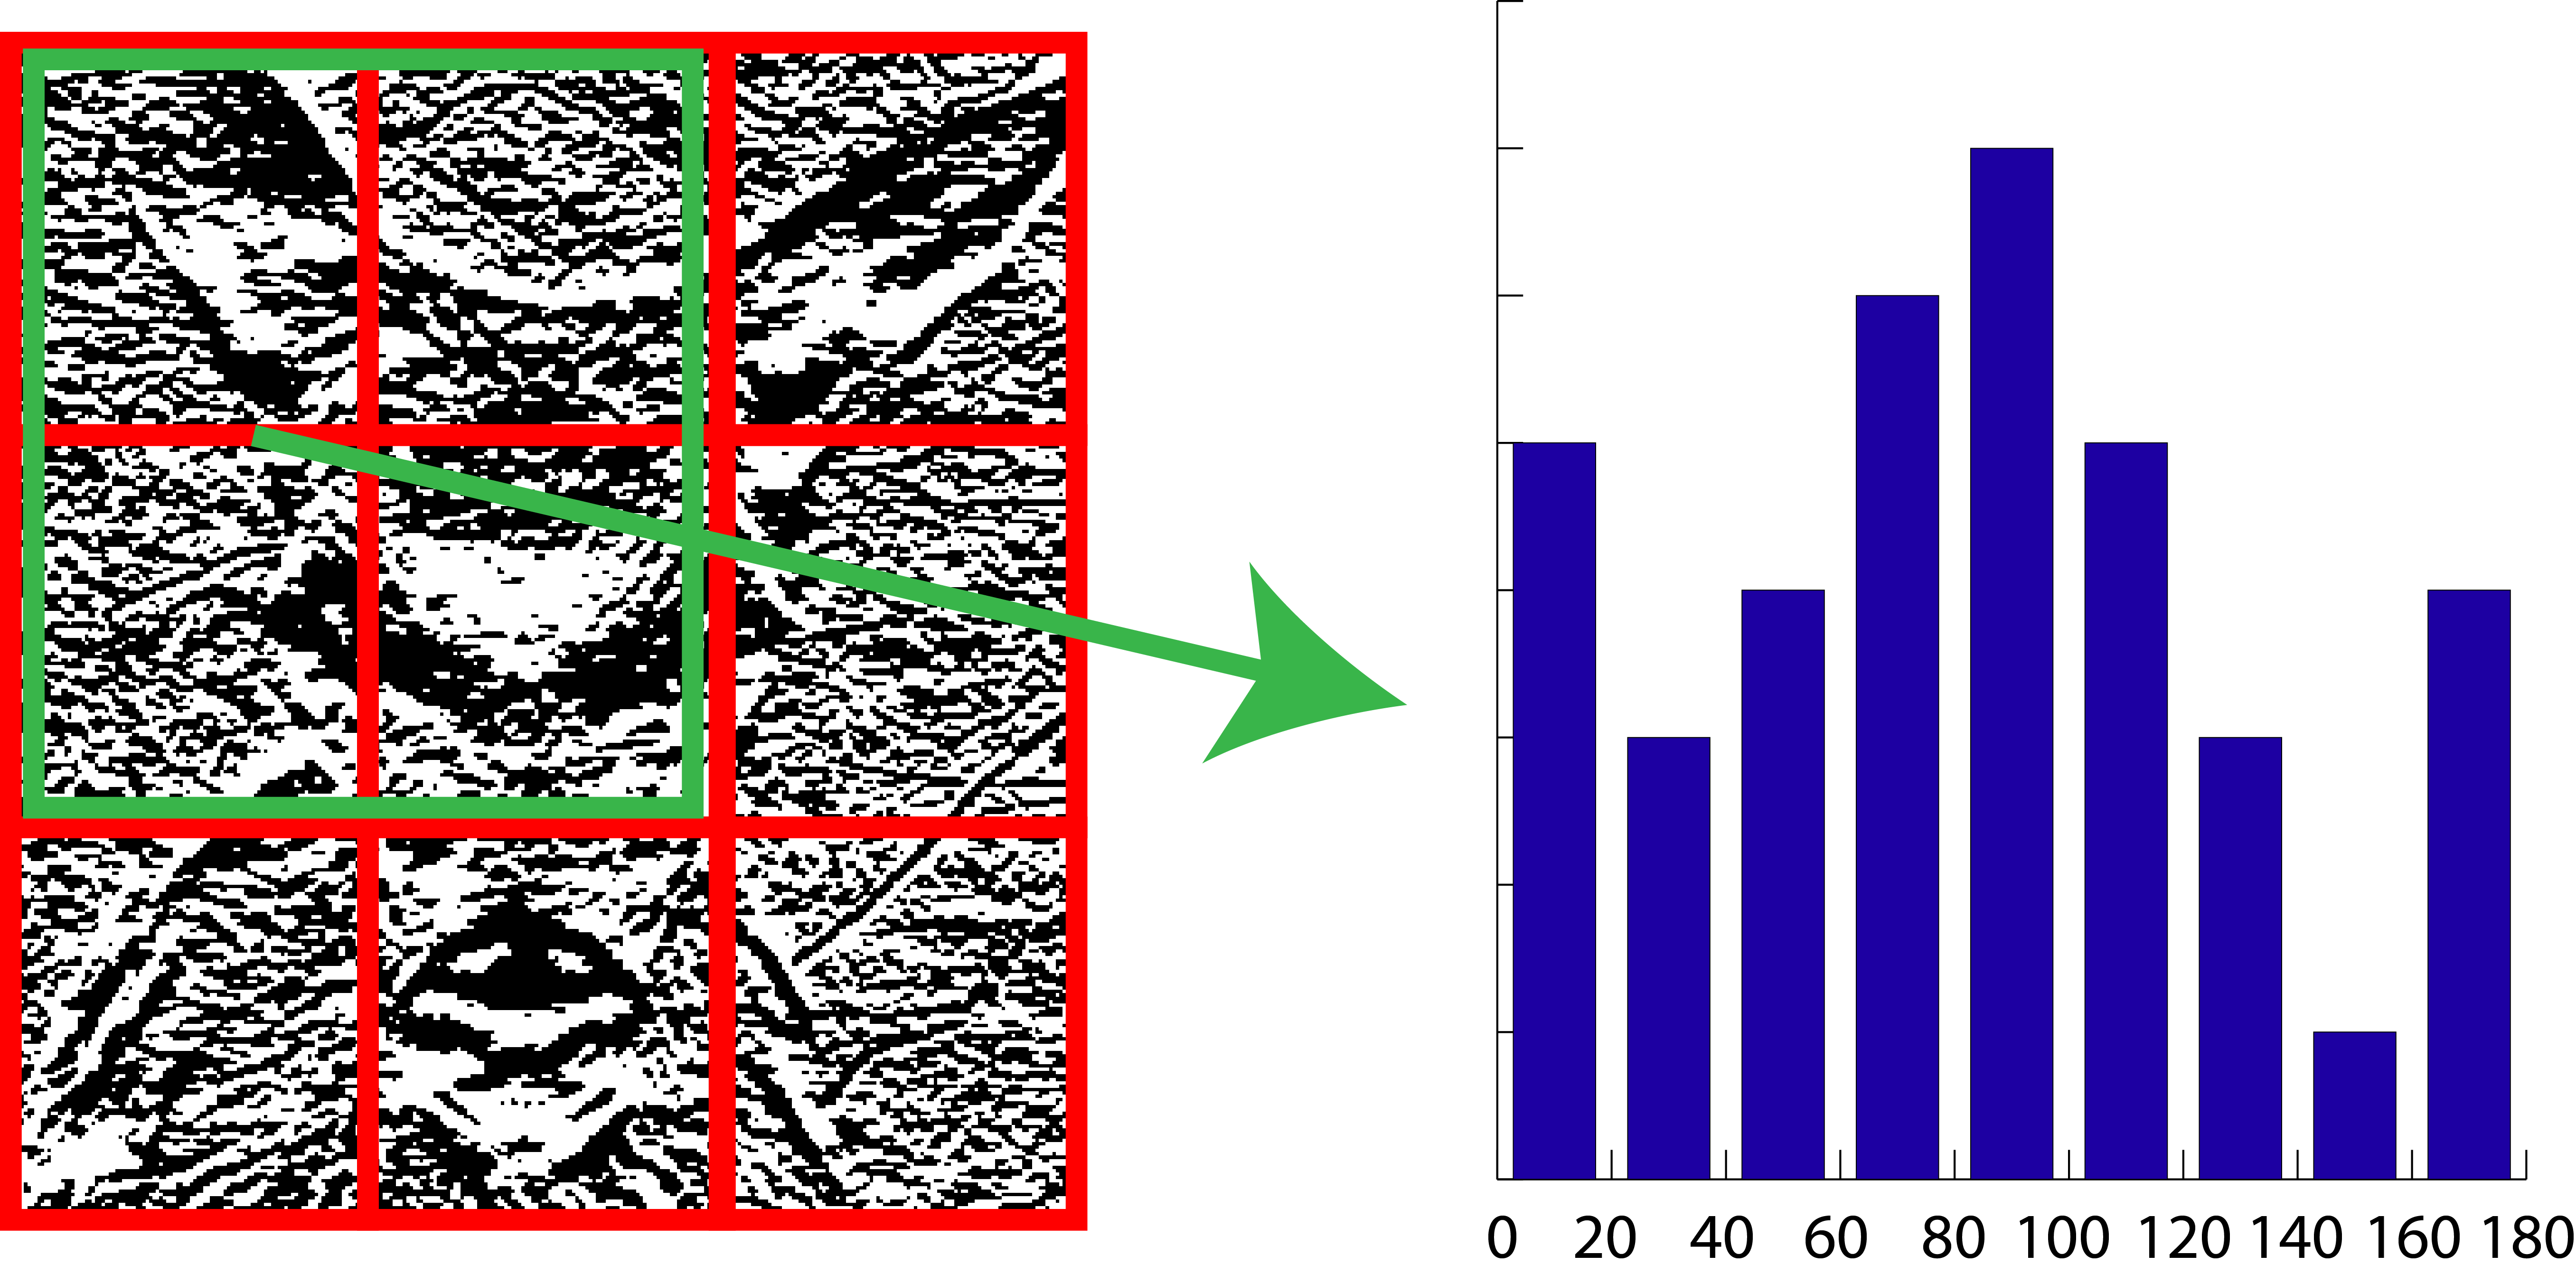
\includegraphics[trim={0 0cm 0cm 0cm},clip=true,width=13cm]{img/sobel2hog.png}
\end{tabular}
\captionof{figure}{Veranschaulichung der Erstellung eines HOG-Deskriptor. Das rote Raster visualisiert die Unterteilung in Zellen. Jeweils vier dieser Zellen werden zusammen als Block betrachtet. So das hier 4 Blöcke möglich wären. Für jeden Block kann dann ein normalisiertes Histogramm erstellt werden. Hier exemplarisch für den grünen Block gezeigt.}
\label{fig:sobel2hog}
\end{center}

IRGENDWO NOCH DARAUF EINGEHEN DAS EINE FESTE PATCH SIZE BENÖTIGT WIRD, DAMIT DIE DESKRIPTOREN GLEICH GROß SIND.

\begin{center}
\begin{tabular}{c}
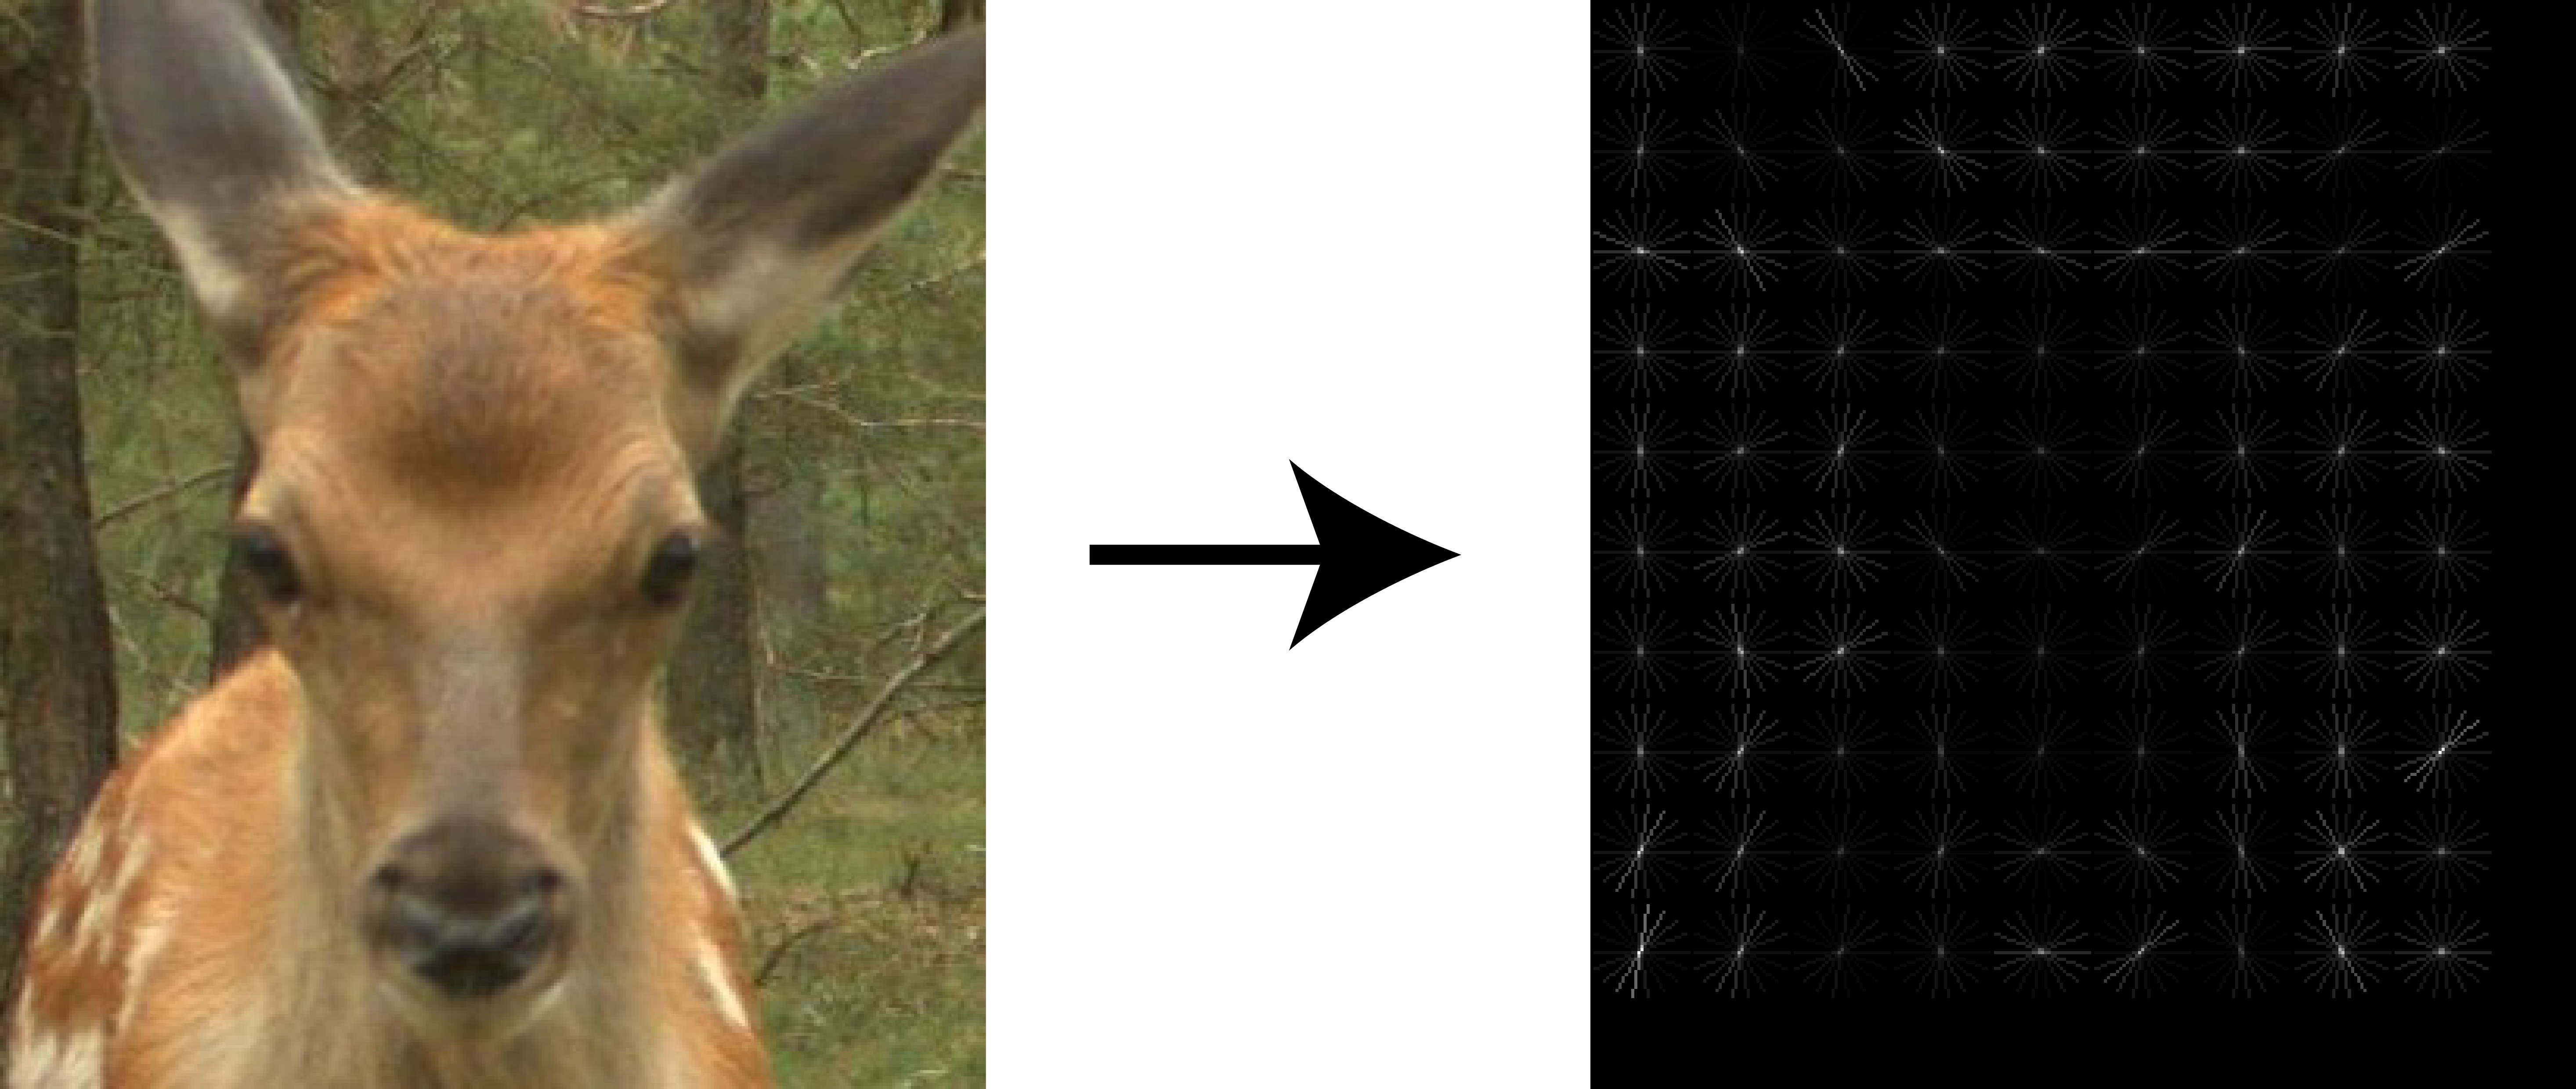
\includegraphics[trim={0 0cm 0cm 0cm},clip=true,width=13cm]{img/Img2HOG.png}
\end{tabular}
\captionof{figure}{Exemplarischer Bildausschnitt (links) und die visuell aufbereitet Repräsentation als HOG-Deskriptor (rechts). In der HOG Repräsentation ist es immer noch möglich das Reh zu erahnen.}
\label{fig:img2HOG}
\end{center}


\subsection{Technische Umsetzung der Klassifizierung}
Umgesetzt wurde der HOG basierte Klassifizierer in Python mit OpenCV (Version: opencv-contrib-python 3.4.2.17). Der Klassifizierer setzt voraus, dass Bilder und die interessanten Regionen (ROI) bereits bestimmt wurden. Details zur ROI Bestimmungen werden in Kapitel~\ref{sec:PCA} gegeben. Die grobe Arbeitsweise wird in Abbildung~\ref{fig:hog_classification_ov} gezeigt. Dabei gibt es zwei Phasen: 1. Training und 2. Klassifikation. Die Trainings Phase wird durch den oberen Verlauf in der Abbildung skizziert. Aus einem gelabeltem Bilder Trainingsdatensatz deren relevanten ROIs selektiert.  Für jedes ROI dieser Bilder wird wie in Abschnitt~\ref{ssec:intro_HOG} erklärt ein HOG-Deskriptor berechnet. Dabei wurde darauf geachtet, dass jedes ROI das selbe Seitenverhältnis besitzt. Zur Beschleunigung der Berechnung wurde der ROI nur als Graustufenbild verarbeitet und auf eine Größe von 128 x 128 Pixel skaliert. Eine Zelle wurde auf 16 x 16 Pixel festgelegt, so das eine Block Größe von 32 x 32 verwendet wurde. Außerdem wurden die Orientierungen auf 9 Gruppen sortiert, so dass eine Richtungsunabhängigge Orientierung betrachtet wurde. Sonstige Parameter des HOG-Descriptors wurden auf den entsprechenden Standardwerten der OpenCV Implementierung belassen. Es wurden mindestens Bild Daten von zwei Tierklassen betrachtet. Die so berechneten und gelabelten Feature Deskriptoren wurden an eine Support Vektor Maschine (SVM) übergeben. Für die SVM wurde eine Radiale Basisfunktion als Kernel gewählt. Experimentell wurden die Parameter $C = 12,5$ und $\gamma = 0,5$ als optimal bestimmt. Details zur Parameter Wahl werden im folgendem Kapitel beschrieben.
Mit Hilfe der so trainierten SVM kann dann in der 2. Phase die Klassifikation der Bilder durchgeführt werden. Dazu werden analog für Bildausschnitte der Testdaten Feature Deskriptoren berechnet und diese von der SVM klassifiziert. Die Qualität dieser Klassifizierung wird im folgendem Unterkapitel beschrieben.
\begin{center}
\begin{tabular}{c}
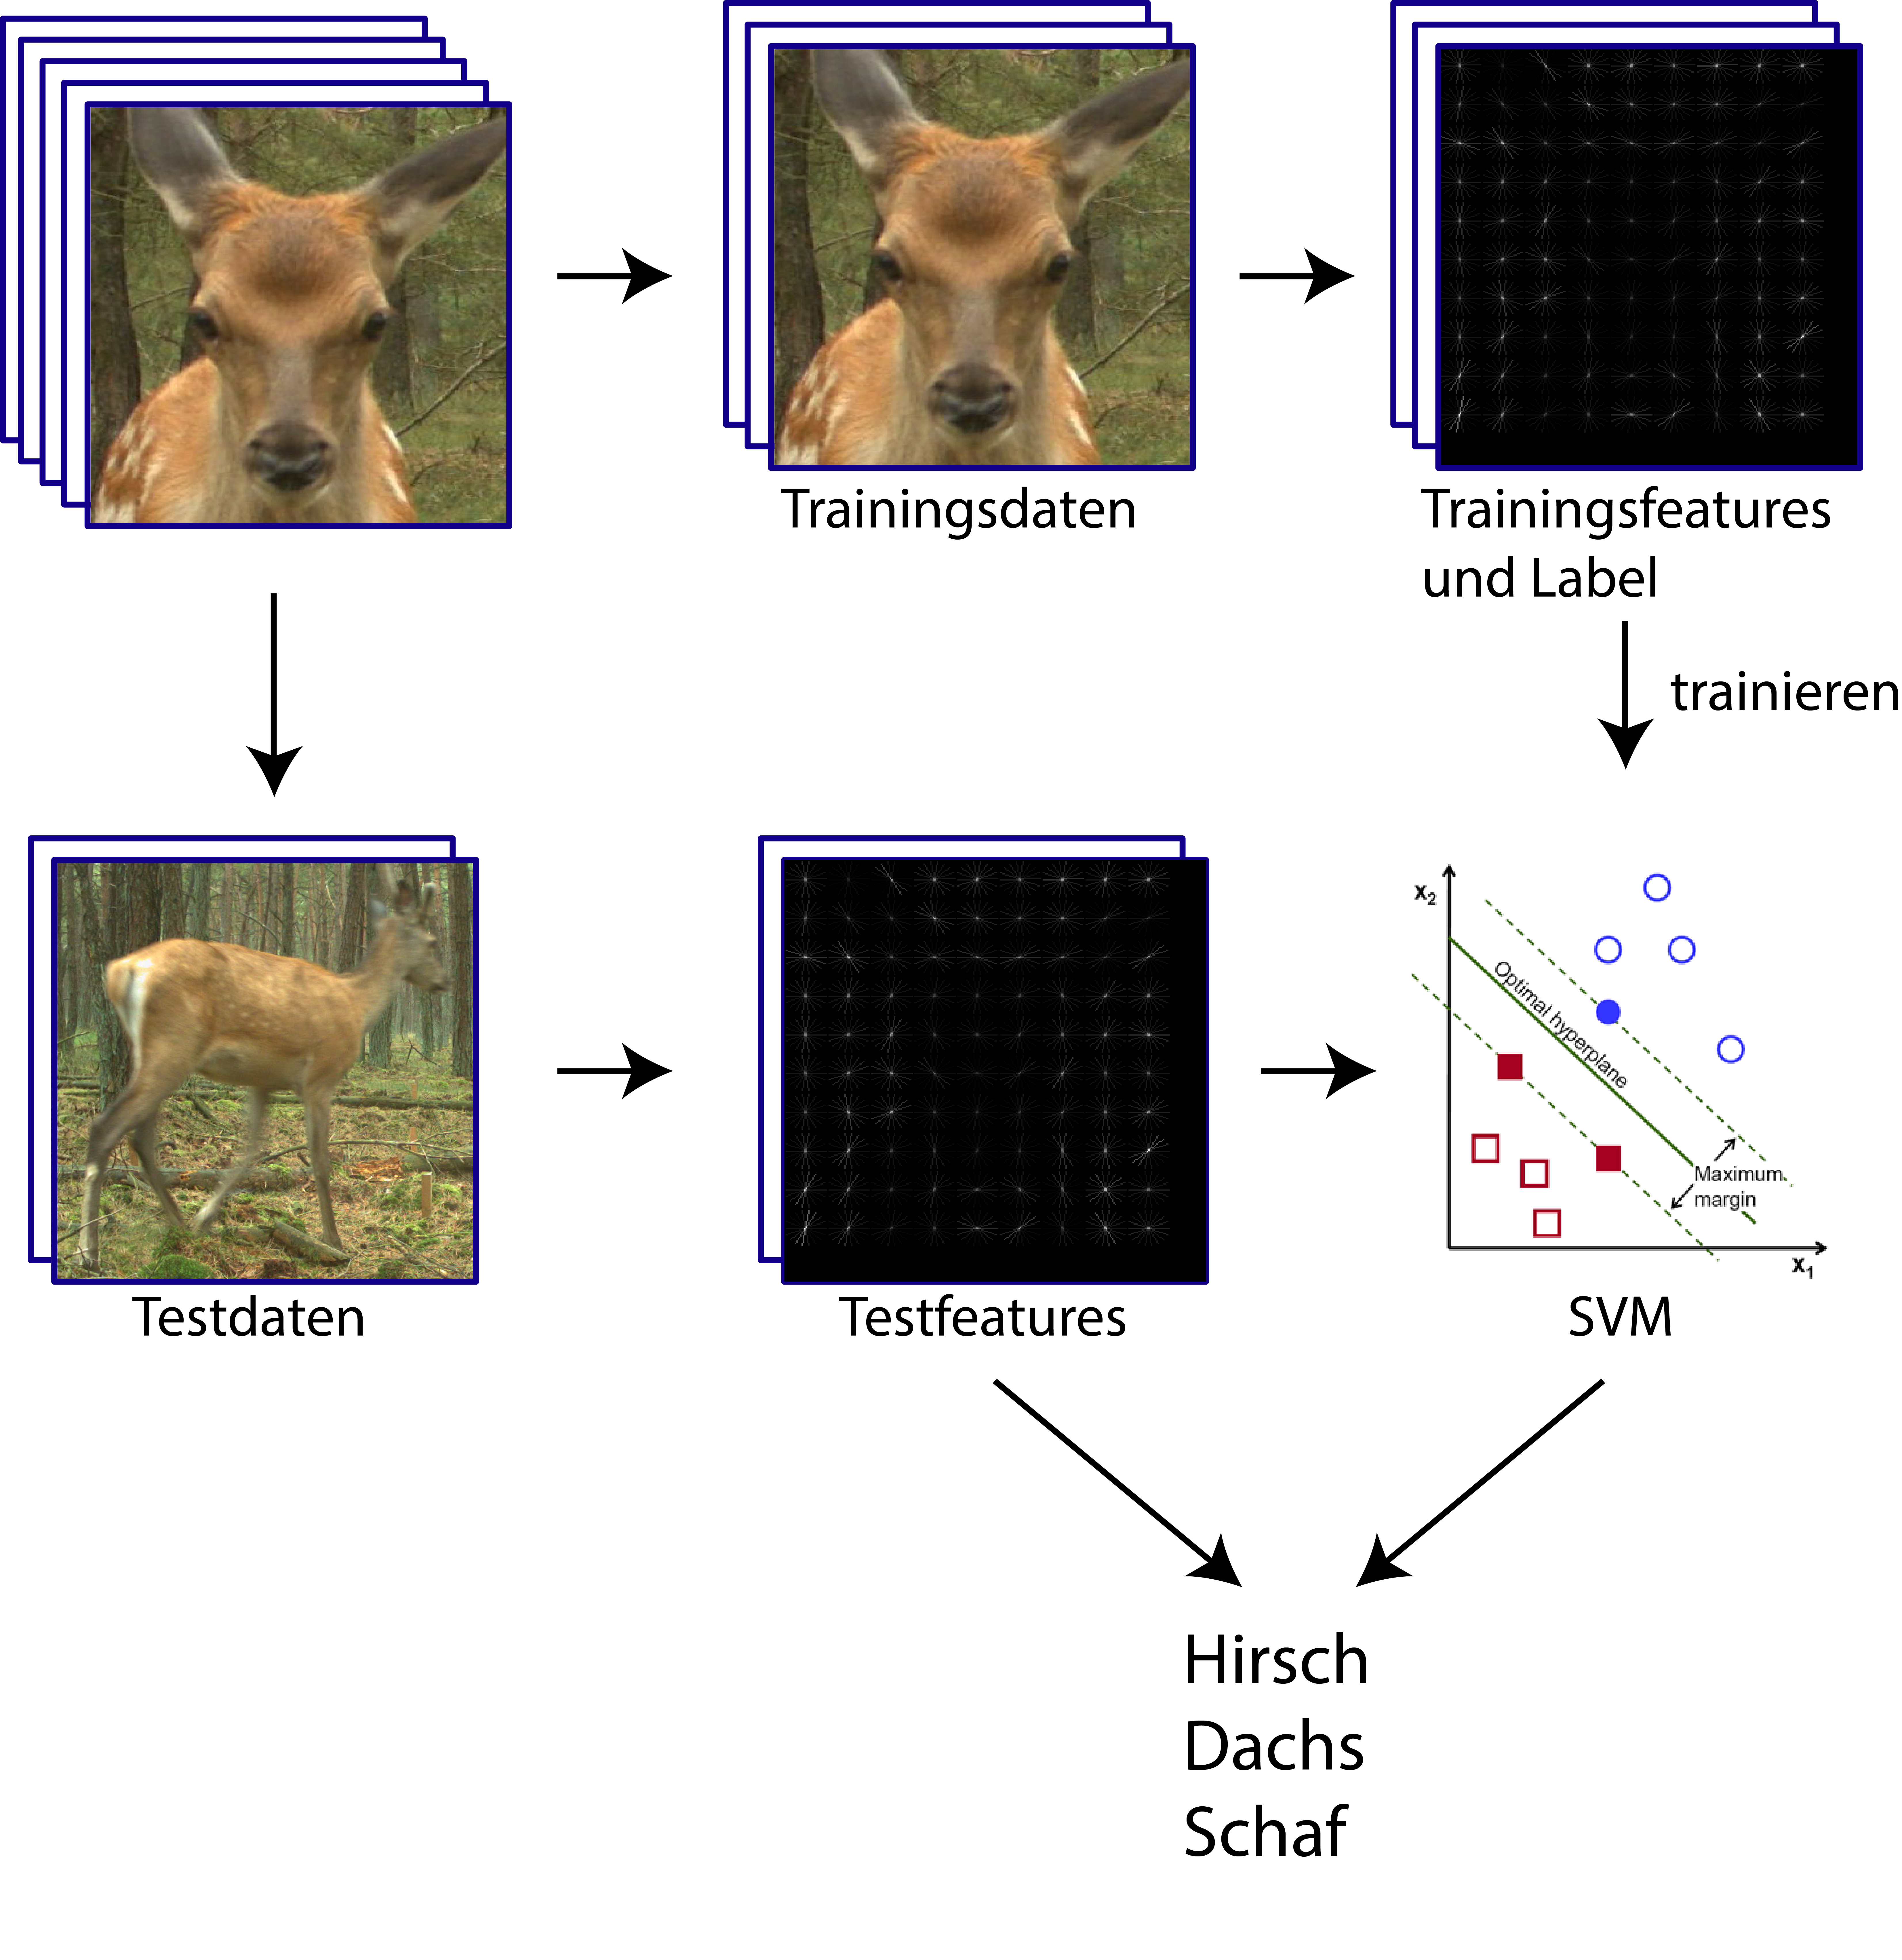
\includegraphics[trim={0 0cm 0cm 0cm},clip=true,width=13cm]{img/ClassificationOverview.png}
\end{tabular}
\captionof{figure}{Schaubild zur Klassifizierung mit einer SVM. Der obere Pfad repräsentiert die Trainingsphase und der untere Pfad die Russifizierungsphase}
\label{fig:hog_classification_ov}
\end{center}


\subsection{Experimentelle Optimierung und Auswertung} \label{sec:HOG_parameter_and_results}
Nur Dachs und Hirsch
Kurze begründung warum!!!!!!!!!!!! 
\subsubsection{Parameterbestimmung HOG-Descriptor und Support Vektor Maschiene}
Einer der wichtigsten Parameter des HOG-Descriptors ist die Größe des betrachteten Bildausschnittes und die Einteilung in Zellen, denn diese Größen bestimmen zum einem die benötigte Rechenzeit, zum anderem aber auch wie viele Details des Bildausschnittes regional aufgelöst werden. Außerdem ergibt sich aus dieser Kombination die Dimension des Ergebnis Vektors. Welche wiederum Einfluss auf den Rechenaufwand der SVM hat. Ziel dieser ersten Parameter Findung was es, die Präzision der Klassifizierung zu maximieren. Dabei wurde jedoch besonders darauf geachtet, dass die Päzision für beide Trainierten Klassen maximal wurde. Dazu wurden die folgenden Größen betrachtet: 64 x 128, 128  x 256, 64 x 64, 128 x 128, 128 x 64 und 256 x 128 Pixeln. Jede dieser Größen wurde einer Zellgröße von 16 x 16 und 32 x 32 Pixeln getestet. Für die Blockgröße wurden jeweils die Kombination aus 4 Zellen verwendet. Die Ergebnisse sind in Tabelle~\ref{tab:HOG_parameter_selection} gezeigt.  

\begin{table}[]
\centering
\caption{Präzision der Klassifizierung abhängig von der Bildausschnitt Größe und der Zellgröße. Es werden aus 50 Zufällig generierten Trainings- und Testdaten Reihenfolgen die jeweils erreichte durschschnittliche Präzision $\overline{p}$, die minimale sowie maximale erhaltene Präzision ($p_{min}, p_{max}$) und die Standardabweichung $\sigma$ angegeben. }
\label{tab:HOG_parameter_selection}
\begin{tabular}{cl}
\hline
\textbf{Ausschnitt [Pixel²]} & \multicolumn{1}{c}{\textbf{Zellgröße 16 x 16}}                                                                                                                                                  \\ \hline
\textbf{64 x 128}                         & \begin{tabular}[c]{@{}l@{}}Dachs: $\overline{p}= 0.913, p_{min}=0.750, p_{max}=1.000, \sigma=0.062$ \\ Damhirsch: $\overline{p}=0.914, p_{min}=0.831, p_{max}=0.987, \sigma=0.034$\end{tabular} \\
\textbf{128 x 256}                      & \begin{tabular}[c]{@{}l@{}}Dachs: $\overline{p}=0.488, p_{min}=0.167, p_{max}=0.833, \sigma=0.161$ \\ Damhirsch: $\overline{p}=0.996, p_{min}=0.949, p_{max}=1.000, \sigma=0.011$\end{tabular}          \\
\textbf{64 x 64}                           & \begin{tabular}[c]{@{}l@{}}Dachs: $\overline{p}=0.908, p_{min}=0.833, p_{max}=1.000, \sigma=0.045 $\\ Damhirsch: $\overline{p}=0.859, p_{min}=0.797, p_{max}=0.916, \sigma=0.035$\end{tabular}          \\
\textbf{128 x 128}                      & \begin{tabular}[c]{@{}l@{}}Dachs: $\overline{p}=0.818, p_{min}=0.500, p_{max}=1.000, \sigma=0.111 $\\ Damhirsch: $\overline{p}=0.951, p_{min}=0.882, p_{max}=0.992, \sigma=0.023$\end{tabular}          \\
\textbf{128 x 64}                        & \begin{tabular}[c]{@{}l@{}}Dachs: $\overline{p}=0.933, p_{min}=0.833, p_{max}=1.000, \sigma=0.050 $\\ Damhirsch: $\overline{p}=0.881, p_{min}=0.709, p_{max}=0.979, \sigma=0.069$\end{tabular}          \\
\textbf{256 x 128}                      & \begin{tabular}[c]{@{}l@{}}Dachs: $\overline{p}=0.675, p_{min}=0.250, p_{max}=1.000, \sigma=0.308 $\\ Damhirsch: $\overline{p}=0.781, p_{min}=0.367, p_{max}=1.000, \sigma=0.249$\end{tabular}          \\ \hline
 & \\
\hline
\textbf{Ausschnitt [Pixel²]} & \multicolumn{1}{c}{\textbf{Zellgröße 32 x 32}}                                                                                                                                                  \\ \hline
\textbf{64 x 128}                         & \begin{tabular}[c]{@{}l@{}}Dachs: $\overline{p}= 0.875, p_{min}=0.750, p_{max}=1.000, \sigma=0.067$ \\ Damhirsch: $\overline{p}=0.854, p_{min}=0.755, p_{max}=0.907, \sigma=0.044$\end{tabular} \\
\textbf{128 x 256}                      & \begin{tabular}[c]{@{}l@{}}Dachs: $\overline{p}=0.883, p_{min}=0.750, p_{max}=1.000, \sigma=0.076$ \\ Damhirsch: $\overline{p}=0.894, p_{min}=0.810, p_{max}=0.928, \sigma=0.037$\end{tabular}          \\
\textbf{64 x 64}                           & \begin{tabular}[c]{@{}l@{}}Dachs: $\overline{p}=0.975, p_{min}=0.917, p_{max}=1.000, \sigma=0.038 $\\ Damhirsch: $\overline{p}=0.859, p_{min}=0.708, p_{max}=0.574, \sigma=0.072$\end{tabular}          \\
\textbf{128 x 128}                      & \begin{tabular}[c]{@{}l@{}}Dachs: $\overline{p}=0.908, p_{min}=0.667, p_{max}=1.000, \sigma=0.102 $\\ Damhirsch: $\overline{p}=0.840, p_{min}=0.705, p_{max}=0.903, \sigma=0.062$\end{tabular}          \\
\textbf{128 x 64}                        & \begin{tabular}[c]{@{}l@{}}Dachs: $\overline{p}=0.967, p_{min}=0.917, p_{max}=1.000, \sigma=0.041 $\\ Damhirsch: $\overline{p}=0.834, p_{min}=0.776, p_{max}=0.932, \sigma=0.045$\end{tabular}          \\
\textbf{256 x 128}                      & \begin{tabular}[c]{@{}l@{}}Dachs: $\overline{p}=0.892, p_{min}=0.833, p_{max}=1.000, \sigma=0.075 $\\ Damhirsch: $\overline{p}=0.867, p_{min}=0.797, p_{max}=1.000, \sigma=0.954$\end{tabular}          \\ \hline
\end{tabular}
\end{table}


\subsubsection{Arten der Testdatengennerierung}
Art der Datenquellen
Einfluss der Datenspiegelung
Generelle Test Parameter

Auswertung (Parameter aus der Vorlesung verwenden


Kapitel Fazit


